\documentclass[11pt]{article}


% -------------------------------------------------
% Packages
% -------------------------------------------------
\usepackage[english]{babel}
\usepackage[
    letterpaper,
    top=2.2cm,
    bottom=2.2cm,
    left=2.5cm,
    right=2.5cm
]{geometry}

\usepackage{amsmath}
\usepackage{amssymb}
\usepackage{booktabs}
\usepackage{graphicx}
\usepackage{float}
\usepackage{caption}
\usepackage{xcolor}
\usepackage{tikz}
\usepackage{pgfplots}
\usepackage{listings}
\usepackage{microtype}
\usepackage[colorlinks=true,allcolors=blue]{hyperref}

\pgfplotsset{compat=1.18}

% -------------------------------------------------
% Formatting
% -------------------------------------------------
\definecolor{lightgray}{gray}{0.94}

\captionsetup{
    font=small,
    labelfont=bf
}

\lstset{
    basicstyle=\ttfamily\small,
    backgroundcolor=\color{lightgray},
    frame=single,
    breaklines=true,
    columns=fullflexible
}

% -------------------------------------------------
% Title
% -------------------------------------------------
\title{
    \textbf{Lorem Ipsum }\\
    \large Placeholder Scientific Article
}

\author{
    Madeline Rodriguez\\ 
    EMSE 368\\
    Case Western Reserve University
}

\date{July 17, 2026\\}

% =================================================
% Document
% =================================================
\begin{document}

\maketitle

% -------------------------------------------------
% Abstract
% -------------------------------------------------
\begin{abstract}
Lorem ipsum dolor sit amet, consectetur adipiscing elit. Integer
pellentesque magna vitae neque gravida, vitae consequat arcu
sollicitudin. Curabitur posuere, sapien sed tincidunt fermentum, neque
massa luctus nisl, a commodo ipsum lectus sed nibh. Praesent elementum
dolor vitae libero posuere, sed pulvinar purus tristique. 
\end{abstract}

\noindent
\textbf{Keywords:}
lorem ipsum; placeholder research; miniature thesis; scientific
formatting; GitHub; Overleaf

% -------------------------------------------------
% Introduction
% -------------------------------------------------
\section{Introduction}

Lorem ipsum dolor sit amet, consectetur adipiscing elit. Nulla facilisi.
Vestibulum posuere ligula sed risus feugiat, eget tincidunt purus
viverra. Sed aliquam, augue vitae consequat fermentum, mauris libero
consequat lectus, at malesuada tortor ligula vitae odio. Donec non
mauris sit amet sem consequat interdum.

Pellentesque habitant morbi tristique senectus et netus et malesuada
fames ac turpis egestas. Duis tristique turpis nec risus volutpat, vel
aliquam mauris vulputate. Etiam in feugiat nisl. Integer porttitor
convallis lectus, vitae vulputate ipsum dignissim non
\cite{placeholder2024}.

% -------------------------------------------------
% Background
% -------------------------------------------------
\section{Background}

Lorem ipsum dolor sit amet, consectetur adipiscing elit. Morbi quis
urna id orci tristique placerat. Suspendisse potenti. Aliquam erat
volutpat. Nam egestas nulla at augue pulvinar, a tristique magna
vulputate. Phasellus id arcu et magna bibendum aliquet.


% -------------------------------------------------
% Research Question and Hypothesis
% -------------------------------------------------
\section{Research Question and Hypothesis}

\subsection{Research Question}

Does increasing the fictional treatment level cause a measurable
increase in the imaginary response value?

\subsection{Hypothesis}

It is hypothesized that the response variable will increase as the
fictional treatment level increases. Lorem ipsum dolor sit amet,
consectetur adipiscing elit. Mauris aliquet tincidunt nibh, sed
facilisis turpis volutpat eget.

% -------------------------------------------------
% Materials and Methods
% -------------------------------------------------
\section{Materials and Methods}

\subsection{Materials}

Lorem ipsum dolor sit amet, consectetur adipiscing elit. The study used
three imaginary specimens, two fictional measurement devices, one
placeholder container, and a collection of synthetic observations.
All materials were selected for demonstration purposes only.

\begin{table}[H]
\centering
\caption{Placeholder materials used in the fictional experiment.}
\label{tab:materials}
\begin{tabular}{lcc}
\toprule
\textbf{Material} & \textbf{Quantity} & \textbf{Purpose} \\
\midrule
Lorem sample A & 3 & Control specimen \\
Ipsum sample B & 3 & Low treatment \\
Dolor sample C & 3 & High treatment \\
Placeholder solution & 500 mL & Exposure medium \\
Imaginary sensor & 1 & Data collection \\
\bottomrule
\end{tabular}
\end{table}

\subsection{Experimental Procedure}

Lorem ipsum dolor sit amet, consectetur adipiscing elit. Each specimen
was placed inside a fictional test chamber for a predetermined period.
The chamber temperature was held at an arbitrary value while the
samples were exposed to three treatment levels.

\subsection{Mathematical Analysis}

The average response was calculated using

\begin{equation}
\overline{x} =
\frac{1}{n}\sum_{i=1}^{n}x_i,
\label{eq:mean}
\end{equation}


The sample standard deviation was calculated using

\begin{equation}
s =
\sqrt{
\frac{\sum_{i=1}^{n}(x_i-\overline{x})^2}
{n-1}
}.
\label{eq:standarddeviation}
\end{equation}

A fictional response model was expressed as

\begin{equation}
R = \alpha T + \beta t + \varepsilon,
\label{eq:model}
\end{equation}

where \(R\) is the imaginary response, \(T\) is the treatment level,
\(t\) is time, \(\alpha\) and \(\beta\) are arbitrary coefficients,
and \(\varepsilon\) represents unexplained variation.

% -------------------------------------------------
% Image and Graphic
% -------------------------------------------------
\subsection{Grayscale Imaging}

Lorem ipsum dolor sit amet, consectetur adipiscing elit. 

\begin{figure}[H]
\centering

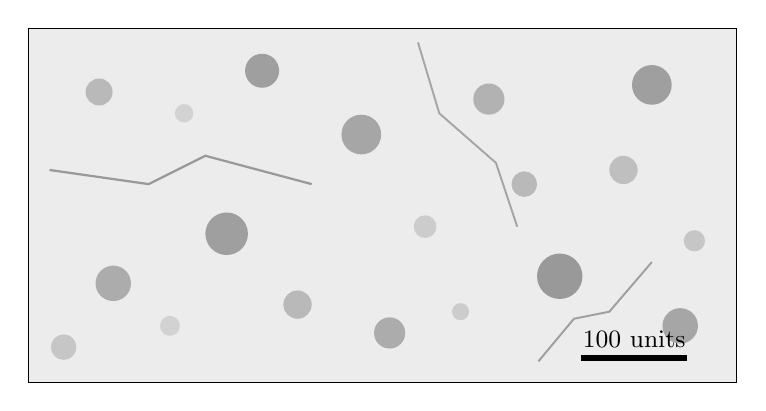
\begin{tikzpicture}[scale=0.9]

\fill[gray!15] (0,0) rectangle (10,5);

\foreach \x/\y/\r/\shade in {
0.5/0.5/0.18/45,
1.2/1.4/0.25/65,
2.0/0.8/0.14/35,
2.8/2.1/0.30/75,
3.8/1.1/0.20/55,
4.7/3.5/0.28/70,
5.6/2.2/0.16/40,
6.5/4.0/0.22/60,
7.5/1.5/0.32/80,
8.4/3.0/0.20/50,
9.2/0.8/0.25/70,
1.0/4.1/0.19/55,
2.2/3.8/0.13/35,
3.3/4.4/0.24/75,
5.1/0.7/0.22/65,
6.1/1.0/0.12/40,
7.0/2.8/0.18/55,
8.8/4.2/0.28/75,
9.4/2.0/0.15/45
}{
    \fill[gray!\shade] (\x,\y) circle (\r);
}

\draw[gray!80, line width=0.8pt]
(0.3,3.0) -- (1.7,2.8) -- (2.5,3.2) -- (4.0,2.8);

\draw[gray!70, line width=0.7pt]
(5.5,4.8) -- (5.8,3.8) -- (6.6,3.1) -- (6.9,2.2);

\draw[gray!75, line width=0.7pt]
(7.2,0.3) -- (7.7,0.9) -- (8.2,1.0) -- (8.8,1.7);

\draw[line width=2pt] (7.8,0.35) -- (9.3,0.35);
\node[above] at (8.55,0.35) {\small 100 units};

\draw[black] (0,0) rectangle (10,5);

\end{tikzpicture}

\caption{
Illustrative grayscale image of a fictional specimen surface. 
}
\label{fig:surface}
\end{figure}

% -------------------------------------------------
% Results
% -------------------------------------------------
\section{Results}

Lorem ipsum dolor sit amet, consectetur adipiscing elit. 

\begin{table}[H]
\centering
\caption{
Fictional mean response values presented as mean
\(\pm\) standard deviation.
}
\label{tab:results}
\begin{tabular}{lccc}
\toprule
\textbf{Time} &
\textbf{Control} &
\textbf{Low Treatment} &
\textbf{High Treatment} \\
\midrule
1 hour  & \(4.1 \pm 0.5\)   & \(18.2 \pm 1.6\)  & \(42.0 \pm 3.2\) \\
6 hours & \(6.5 \pm 0.7\)   & \(31.4 \pm 2.1\)  & \(76.5 \pm 5.8\) \\
24 hours& \(9.8 \pm 1.0\)   & \(52.3 \pm 4.0\)  & \(119.7 \pm 8.4\) \\
72 hours& \(12.6 \pm 1.4\)  & \(68.1 \pm 5.2\)  & \(161.3 \pm 10.1\) \\
\bottomrule
\end{tabular}
\end{table}

Figure~\ref{fig:resultsgraph} displays the same placeholder values in
graphical form. The use of different symbols and line patterns allows
the figure to remain readable when printed in grayscale.

\begin{figure}[H]
\centering

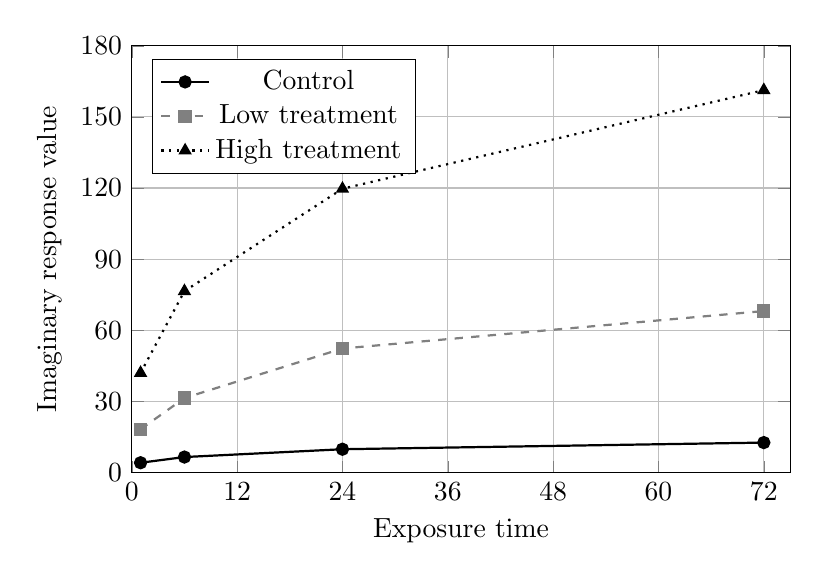
\begin{tikzpicture}
\begin{axis}[
    width=0.82\textwidth,
    height=7cm,
    xlabel={Exposure time},
    ylabel={Imaginary response value},
    xmin=0,
    xmax=75,
    ymin=0,
    ymax=180,
    xtick={0,12,24,36,48,60,72},
    ytick={0,30,60,90,120,150,180},
    grid=major,
    legend style={
        at={(0.03,0.97)},
        anchor=north west,
        draw=black,
        fill=white
    },
    mark options={solid}
]

\addplot[
    black,
    mark=*,
    thick
]
coordinates {
    (1,4.1)
    (6,6.5)
    (24,9.8)
    (72,12.6)
};
\addlegendentry{Control}

\addplot[
    gray,
    mark=square*,
    thick,
    dashed
]
coordinates {
    (1,18.2)
    (6,31.4)
    (24,52.3)
    (72,68.1)
};
\addlegendentry{Low treatment}

\addplot[
    black,
    mark=triangle*,
    thick,
    dotted
]
coordinates {
    (1,42.0)
    (6,76.5)
    (24,119.7)
    (72,161.3)
};
\addlegendentry{High treatment}

\end{axis}
\end{tikzpicture}

\caption{
Fictional relationship between treatment time and the imaginary
response variable.
}
\label{fig:resultsgraph}
\end{figure}

The high-treatment group reached a maximum fictional response of 161.3
units after 72 hours. In comparison, the control group reached only
12.6 units. These values are entirely fabricated and exist only to
demonstrate proper scientific data presentation.

% -------------------------------------------------
% Discussion
% -------------------------------------------------
\section{Discussion}

Lorem ipsum dolor sit amet, consectetur adipiscing elit. Curabitur
lobortis tincidunt elit, vitae suscipit sem tincidunt sed. Donec
elementum massa vitae ex viverra, sed elementum augue molestie. The
fictional findings appear to support the stated hypothesis because the
response increased with treatment level.

The apparent relationship may be explained by an imaginary interaction
between the specimen and the treatment medium. Sed posuere velit in
erat consectetur, vel faucibus lacus consectetur. Integer euismod
tortor non dolor sollicitudin, ac dictum risus interdum
\cite{example2023}.


% -------------------------------------------------
% Limitations
% -------------------------------------------------
\section{Limitations}

Lorem ipsum dolor sit amet, consectetur adipiscing elit. 

% -------------------------------------------------
% Conclusion
% -------------------------------------------------
\section{Conclusion}

Lorem ipsum dolor sit amet, consectetur adipiscing elit.

% -------------------------------------------------
% Version Control
% -------------------------------------------------
\section{Backup and Version-Control System}

The project source files were backed up using Git and GitHub. Git tracks
changes to the \LaTeX{} source file, while GitHub stores a remote copy
of the repository. This system allows earlier versions of the document
to be restored and provides evidence that the project has been backed
up.


\noindent
\textbf{Git clone address:}
\begin{center}
\url{https://git@git.overleaf.com/6a5d5b70b7a3a347771ccd97}
\end{center}
\textbf{GitHub repository address:}

\begin{center}
\url{https://github.com/mrr146-ops/sync}
\end{center}

% -------------------------------------------------
% Acknowledgments
% -------------------------------------------------

% -------------------------------------------------
% References
% -------------------------------------------------
\begin{thebibliography}{9}

\bibitem{placeholder2024}
A. Author and B. Researcher.
``A Placeholder Investigation of Imaginary Scientific Variables.''
\textit{Journal of Fictional Research},
vol. 12, no. 3, pp. 100--110, 2024.

\bibitem{example2023}
C. Scientist.
\textit{Methods for the Analysis of Nonsensical Experimental Data}.
Example Academic Press, 2023.

\bibitem{formatting2022}
D. Writer and E. Editor.
``Scientific Formatting in Miniaturized Documents.''
\textit{International Review of Placeholder Studies},
vol. 8, no. 2, pp. 44--59, 2022.

\end{thebibliography}

\end{document}

